\begin{figure}[H]
\centering
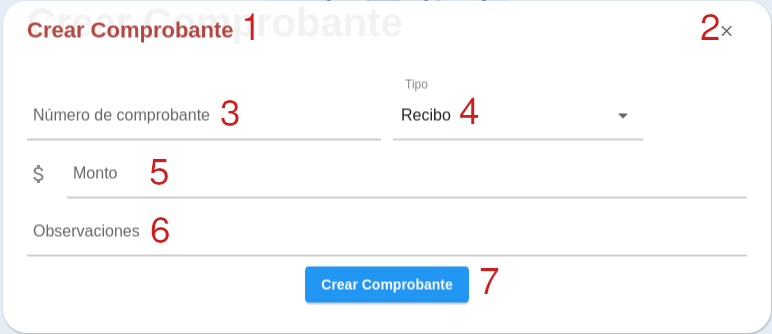
\includegraphics[width=\textwidth,height=\textheight,keepaspectratio]{Escenarios/AD-15-00}
\caption{Escenario - AD-15-00}
\label{fig:AD-15-00}
\end{figure}
Este es el escenario que permite a los usuarios crear y modificar comprobantes, el campo \textbf{AD-15.01} indicará la acción que se va a realizar, pudiendo ser 'Crear comprobante' o 'Editar comprobante'. Con el botón \textbf{AD-15-02} se podrá cerrar la ventana y volver al escenario \textbf{AD-14-00}.
En el campo \textbf{AD-15-03} el usuario debe especificar el número del comprobante. La lista desplegable \textbf{AD-15-04} le permite al usuario elegir el tipo de comprobante. En el campo \textbf{AD-15-05} el usuario debe especificar el monto del comprobante. En el campo \textbf{AD-15-06} el usuario podrá especificar las observaciones que considere. Si el usuario hace click en el botón \textbf{AD-15-08} creará o modificar el comprobante y navegará al escenario \textbf{AD-14-00}.
\\